%=============================================================================
% THIS IS chapter{WMC Tool: Automatic instrumentation of floating-point speech
% and audio codecs for complexity and memory measurements
% 
% Jan.2023 - created by Vladimir Malenovsky
%=============================================================================
\chapter{WMC Tool: Automatic instrumentation of floating-point speech
         and audio codecs for complexity and memory measurements}
%=============================================================================

%-----------------------------------------------------------------------------
\section{Introduction}

The WMC tool performs automatic instrumentation of speech and audio codecs written in floating-point C code to measure their computational complexity and memory. The WMC tool is an extension of the \nameref{ch:cmplx_eval_tool} described in Chapter \ref{ch:cmplx_eval_tool}. The WMC tool uses its own set of pseudo-instructions and wrapper functions that are build on top of the complexity measurement counters (macros) defined in Table \ref{tbl:flp-counters}. The complexity of functional blocks is evaluated by inserting a pair of special functions at the beginning of the function and at the end of the function. The WMC tool measures the minimum, the maximum and the average complexity in WMOPS (Weighted Million OPerations per Second) by defining the number of frames per second.

The WMC tool inserts special functions at the end of each \verb|.c| file to calculate the Program ROM and Data (Table) ROM. The Program ROM is estimated by counting the total number of instructions in the source file. The Data ROM is estimated by counting the total size of all constant variables in the source file.

The Data RAM consumption is measured by monitoring all stack and heap allocations and tracking their maximum values. To find the maximum stack consumption the WMC tool inserts special macros at the beginning and at the end of each function call and monitors the pointer to the bottom of the stack. To estimate the maximum heap consumption the WMC tool instruments all calls to \verb|malloc()|, \verb|calloc()| and \verb|free()| standard functions.

The WMC tool may optionally insert code to print summary information about both computational complexity and memory consumption. Note, that the WMC tool provides only an estimate of the computational complexity and memory consumption. The measured numbers shall not be directly compared to the fixed-point counterpart of the algorithm under test. The WMC tool does not account e.g. for the scaling (normalization) of variables, saturation or overflow control. The measured complexity is also influenced by the programming style, for example the usage of pointer dereferencing, complex structures, custom data declarations, etc.

%-----------------------------------------------------------------------------
\section{Description of the WMC Tool}

The WMC tool can be used only on \verb|.c| source files following the C89/C90 ISO standard \cite{C90}. The WMC tool will not work with other languages nor will it understand C++ source files. The WMC tool reads and parses all \verb|.c| files matching the file mask provided on the command line. If the files were previously instrumented, the inserted pseudo-isntructions are first all removed. Then, all source files are re-instrumented again. The source files are modified in place  after being backed up before processing. The instrumented source files may be compiled and linked with other source files and libraries of the project. 

\subsection{Usage}
\label{ch:usage_wmc_tool}

The WMC tool package contains the following files:

\begin{itemize}
    \item \verb|wmc_tool.cpp|: Main program
    \item \verb|c_parser.cpp|: Routines for parsing C functions
    \item \verb|text_utils.cpp|: Text and string processing functions
    \item \verb|output.cpp|: Warning and error messages
    \item \verb|wmc_auto_h.txt|: Auto-generated header file for inclusion in projects
    \item \verb|wmc_auto_c.txt|: Auto-generated C source file for inclusion in projects
\end{itemize}

Note, that the files \verb|wmc_auto_h.txt| and \verb|wmc_auto_c.txt| contain the definitions of WMC complexity and memory counting functions in the raw text format. The WMC tool converts these files in the platform-specific format to be included as part of the user project. These files shall not be modified by an any external program or converted manually.

The WMC tool uses the following mandatory and optional arguments.

\begin{Verbatim}[fontsize=\scriptsize]
Mandatory arguments:
    space-separated list of filenames or directories with file mask, e.g. ./lib_code/array*.c
    note: if file mask is not specified *.c is assumed by default
Options:
    -h [--help]: print help
    -v [--verbose]: print warnings and other information messages
    -i [--info-only]: only print instrumentation information
    -d [--desinstrument]: desintrument only
    -m filename [--rom filename]: add statistics about ROM and RAM consumption
        note: filename shall point to a .c file containing the print_mem() function
    -b [--no-backup]: no backup of original files
    -c dirname [--generate-wmc-files dirname]: copy wmc_auto.h and wmc_auto.c to a user-specified directory
\end{Verbatim}

\subsection{Instrumentation process}
\label{ch:instrumentation_process}

The WMC tool may be applied on individual \verb|.c| files or entire directories containing \verb|.c| files. The examples below illustrate the usage of the WMC tool on Unix-based platforms.

To instrument a file named \verb|test.c| the WMC tool shall be used as follows:

\verb|./wmc_tool test.c|

To instrument \verb|.c| files in a directory named \verb|lib_code| the WMC tool shall be used as follows:

\verb|./wmc_tool "lib_code/*.c"|

Note, that on Unix-based platforms it's necessary to use the \verb|""| quotes when specifying file masks on the command-line to avoid globing. 

The WMC tool uses the C header file named \verb|wmc_auto.h| and the C source file named \verb|wmc_auto.c| to interpret the instrumented code. Therefore, the files \verb|wmc_auto.h| and \verb|wmc_auto.c| \textbf{must} be included in the project and made visible to all instrumented source files. In fact, the C header file \verb|wmc_auto.h| is included by the WMC tool automatically, if not already included in the instrumented C source file. This is done with the following definition.

{
{\em /*AddedByWMC\_Tool*/}    {\verb|#include "wmc_auto.h"|}
}

The files \verb|wmc_auto.h| and \verb|wmc_auto.c| may be copied from one project to another as they are not project-specific. In case that the files \verb|wmc_auto.h| and \verb|wmc_auto.c| are missing or corrupted, it is possible to re-create them by the WMC tool using the \verb|-c| command-line option.

The WMC instrumentation process is illustrated on the schematic diagram in \ref{fig:wmc_tool_general}. The details of the individual processing blocks are described in the following text.

\begin{figure}[!hbtp]
\begin{center}
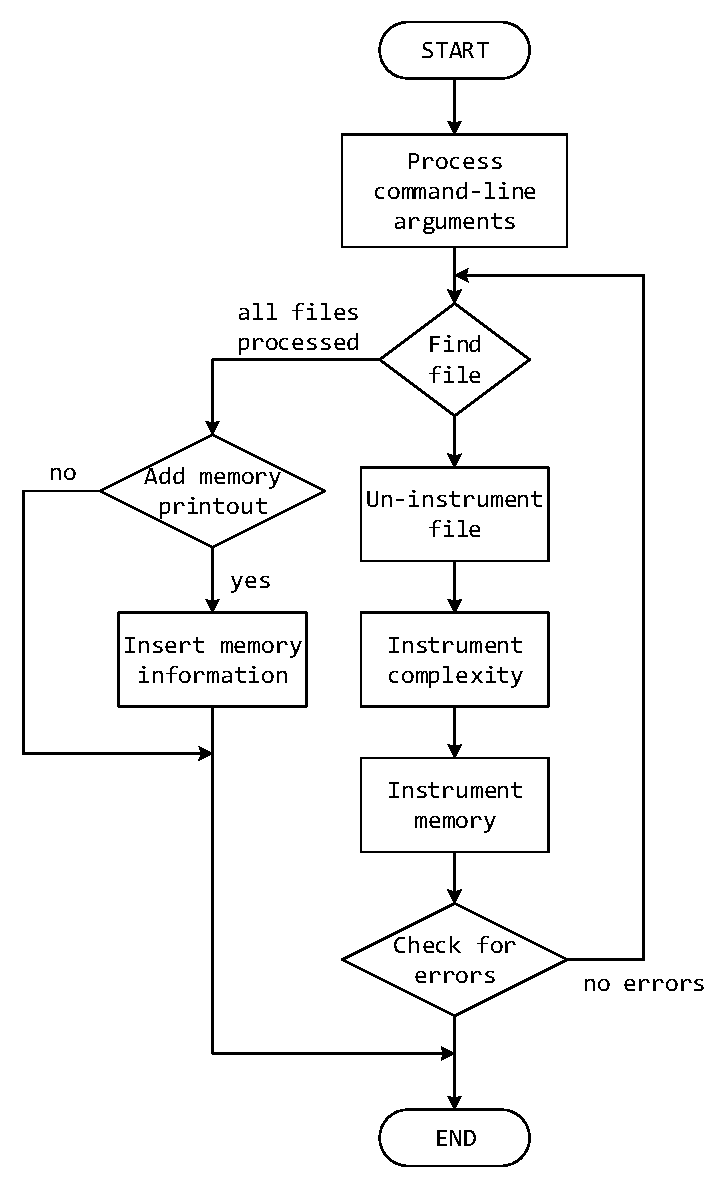
\includegraphics[width=11.8cm,keepaspectratio]{wmc_tool_general}
\end{center}
\caption{The WMC instrumentation process}
\label{fig:wmc_tool_general}
\end{figure}

%-----------------------------------------------------------------------------
\subsubsection{Errors}

Since the WMC tool modifies source files it is necessary that they can still be compiled successfully after instrumentation. The WMC tool is strict and will not process a source file that cannot be compiled. Any error encountered during the un-parsing process, un-instrumentation process or re-instrumentation process will stop any further progres. The source file will be unchanged unless the error occurred during writing operation. In that case, the source file might be partially modified. When specifying more than one source file on the command line the source files processed prior to the one where error occured will be instrumented while the remaining files will not.
	
%-----------------------------------------------------------------------------
\subsubsection{Warnings}

Warnings are issued when the WMC tool detects certain conditions in a source file. By default, no warnings are printed on the screen during the processing unless the WMC tool is invoked in the verbose mode by specifying the \verb|-v| option on the command line. Absent from any errors the processing will continue and the source file will be instrumented. The WMC tool is designed to give as much feedback as possible. All warnings can be safely ignored but correcting them in the source file usually helps the tool to instrument the statements better and more closely to their fixed-point counterpart. 

Note, that the WMC tool is not a perfect C parser. It might issue an error even on certain valid instructions and statements. For example, the WMC tool has no knowledge of global constants and macros (\verb|#define|) declared in \verb|.h| include files because it does not open them. The WMC tool cannot detect all forms of complex function calls and pointer de-references and it does not recognize custom data types directly. A more detailed description of the limitations of the WMC tool can be found in Section \ref{ch:limitations}.

%-----------------------------------------------------------------------------
\section{Instrumentation of complexity}
\label{ch:instrumentation_of_complexity}

The WMC tool only instruments functions but not macros. System functions and functions with names that are considered as basic operations are skipped. The instrumentation mechanism has been designed to be as least intrusive as possible. The instrumentation code is inserted at the beginning of each instrumented line in the source code with a single macro that has the following form \verb|$("ops")| where \verb|ops| is a string of letters and symbols indicating individual operations. The WMC tool parses each source file and calculates the length of each instrumentation string. The maximum length is then used to indent the entire source file to make space for the instrumentation strings. This is shown in the example below. 

\begin{Verbatim}[fontsize=\small]
    float calc_shift_value( const float totalStep )
    { func_start_
        float sdf, reset_value;

$("M")  reset_value = 0.23f;
$("Gt") if_( totalStep > 23.3456f )  
        {
$("M**-")   reset_value = 56.345e-4f * (float)exp_( 34.456 * totalStep ) \\
                          - 2.65f;
        }

        return_ reset_value;
    }
\end{Verbatim}

It is always possible to remove the instrumentation from the source code with the \verb|-d| command line option. In many cases, the source file will then return to its original non-instrumented state except for whitespace characters and text alignment. The un-instrumentation process is also invoked automatically by the WMC tool as the first step in the instrumentation process. This ensures that the results are identical even when the process is repeated multiple times. This allows the users to make modifications to an already instrumented source code by simply re-instrumenting it again. Note, that the un-instrumentation process does not remove the functions \verb|push_wmops()| and \verb|pop_wmops()| and the system functions. Lines that are preceded by

{
{\em /*AddedByWMC\_Tool*/} 
}

are removed completely. At the end of the un-instrumentation process, the original indentation is restored.

If, for any reason, it is necessary to avoid the automatic instrumentation and un-instrumentation of certain parts in the source code, the user may encapsulate such parts in \verb|#define WMC_TOOL_SKIP| \ldots \verb|#undef WMC_TOOL_SKIP| macro pairs. For example

\begin{Verbatim}[fontsize=\small]
#define WMC_TOOL_SKIP
    p_dir_out_region = (float *) malloc( sizeof( h_Out_Region * m_outputs );
#undef WMC_TOOL_SKIP
\end{Verbatim}

%-----------------------------------------------------------------------------
\subsection{Keywords}

Keywords in the source code are instrumented by appending the underscore '\verb|_|' symbol to the ir name. The following table demonstrates the instrumentation of the most common keywords.

\begin{table}
\raggedleft\small
\caption{Instrumentation of keywords}
\begin{tabular}{|l|p{0.2\textwidth}<{\raggedright}|p{0.6\textwidth}<{\raggedright}|}
\hline
\textbf{Keyword} & \textbf{Instrumented as} & \textbf{Comments} \\
\hline
\verb|while (cond)| & \verb|while_ (cond)| & \\
\hline
\verb|case| & \verb|case| & The keyword itself is not instrumented but a \verb|cost(n)| instrumentation macro will be inserted after the semi colon '\verb|:|'. The value of '\verb|n|' is initialized to 1 and increases with each additional case inside the \verb|switch| block. Note, that the value of '\verb|n|' is re-initialized to 1 in each nested \verb|switch| block. \\
\hline
\verb|default| & \verb|default| & Same as \verb|case|. \\
\hline
\verb|switch| & \verb|switch| & In case there are is no \verb|default| keyword in the \verb|switch| block a \verb|cost(n)| instrumentation macro will be inserted after the closing brace '\verb|}|'. \\
\hline
\end{tabular}
\label{tab:instrumentation_of_keywords}
\end{table}

The following example demonstrates the instrumentation of the \verb|switch/case/default| keywords. 

\begin{Verbatim}[fontsize=\small]
    switch_( fruit_type )
    {
        case APPLE:cost_(1)
        case ORANGE:cost_(2)
        case BANANA:cost_(3)
        {
$("Lt")     if_( fruit_cost < 490.5f )
            {
$("M")          mood = 0;
            }
            else $("Lt")if_( fruit_cost < 660.8f )
            {
$("M")          mood = 1;
            }
            else
            {
$("M")          mood = 2;
            }
            break_;
        }
        default:cost_(4) 
        {
            switch_ (old_fruit_type)
            {
                case APPLE:cost_(1)
                case BANANA:cost_(2)
                {
$("M")              mood = 2;
                    break_;
                }
            }cost_(3)
        }
    }
\end{Verbatim}

For more information on keywords that are \textbf{NOT} instrumented invoke the WMC tool with the \verb|-i| command-line option.

%-----------------------------------------------------------------------------
\subsection{Mathematic functions}

The most common mathematic functions defined in \verb|math.h| are instrumented by appending an underscore '\verb|_|' to their name. As the definition of these functions (the function body) is part of the standard C library the complexity cost associated with these functions is pre-calculated and defined within the WMC tool itself as follows

\begin{table}[!hb]
\centering\small
\caption{Complexity cost of mathematic functions}
\begin{tabular}{|l|l|} 
\hline
\textbf{Name} & \textbf{Cost} \\
\hline
\verb|abs()| and its derivatives & 1 \\
\verb|min()| and \verb|max()| & 1 \\
\verb|floor()| & 1 \\
\verb|sqr()| & 1 \\
\verb|sign()| & 1 \\
\verb|round()| & 0 (not supported by the WMC tool) \\
\verb|sqrt()| and \verb|inv_sqrt()| & 10 \\
\verb|log()|, \verb|log2()| and thier derivatives & 25 \\
\verb|exp()| and \verb|pow()| & 25 \\
\verb|sin()|, \verb|cos()| and all other trigonometric functions & 25 \\
\hline
\end{tabular}
\label{tab:cost_of_math_functions}
\end{table}

%-----------------------------------------------------------------------------
\subsection{User-defined functions}

All user-defined functions in the source code are instrumented with one or more underscore '\verb|_|' symbols appended to their names. The WMC tool will count the number of arguments from the function call and insert a wrapper macro at the top of the source file, after the first \verb|#include| section. See the example below.

\begin{Verbatim}[fontsize=\small]
#include <stdlib.h>
#include <sfruits.h>
/*AddedByWMC_Tool*/#define Get_Value_TBX_ func_(Get_Value_TBX,1)

        float Initiate_process( float bgf )
        { func_start_
            float ftrm, result;

$("M")      ftrm = 0;
$("+=")     ftrm += bgf * 5.48f;

            result = Get_Value_TBX_( ftrm );

            return_ result;
        }
        
        float Get_Value_TBX( float tied_state )
        { func_start_
            float ff;

$("M*")     ff = tied_state * 5.44f;

            return_ ff;
        }
\end{Verbatim}

The WMC tool appends an additional underscore symbol '\verb|_|' in each variant of the user-defined function call. This means that if a function is defined to accept a variable number of arguments the first function call will have one underscore symbol '\verb|_|' appended to its name, the second function call will have two underscore symbols '\verb|__|' appended to its name and so on. The WMC tool supports up to 10 variants (different number of arguments) of the same function.

%-----------------------------------------------------------------------------
\subsection{Operators}

The WMC tool divides the operators in three categories as follows.

\begin{table}[!hb]
\centering\small
\caption{Instrumentation of operators}
\begin{tabular}{|c|c|c|} 
\hline
\textbf{Category} & \textbf{Operator} & \textbf{Instrumented as} \\
\hline
Logical operators & '\verb|&&|' and '\verb$||$' & '\verb|__|' double uderscore appended \\
\hline
Ternary operators & '\verb|?|' and '\verb|:|' & '\verb|_|' single uderscore appended \\
\hline
Other operators & '\verb|*,%,<<,+=,...|' & '\verb|$("...")|' wherever appropriate \\
\hline
\end{tabular}
\label{tab:instrumentation_of_operators}
\end{table}

Only the operators from the last category are instrumented by means of the '\verb|$("...")|' instrumentation macro inside the left margin. When an operator is used in the \verb|for| or \verb|while| loop control statement the WMC tool will instrument that operator twice. The first time it will be before the control statement and the second time it will be somewhere inside the loop body. This is demonstrated in the example below

\begin{Verbatim}[fontsize=\small]
      void main(void)
      {
          int a = 0;
$("+=Le") while_ (a+=1 <= 10)
$("+=Le") {
              printf("%i\n", a);
          }
      }
\end{Verbatim}

The WMC tool always tries to insert the instrumentation macro at the least intrusive place in the code but. However, sometimes the WMC tool will be forced to insert the instrumentation macro between two keywords such as in the following example.

\begin{Verbatim}[fontsize=\small]
      void main(void)
      {
$("Ee")   if_ (a==10)
$("*=")       a*=2;
          else $("Lt")if_ (a<10)
          {
$("<<=")      a<<=2;
          }
      }
\end{Verbatim}

The WMC tool will keep the source code aligned. If there is no space to insert the \verb|$("...")| instrumentation macro, the whole source file will be right shifted by a multiple of 4 space characters to accommodate the insertion. This also suggests a useful hint that programmers should write the source code by setting the Tab size to 4 spaces and replace all Tab characters with spaces.

The operators are instrumented by following the set of the following rules.

\begin{table}[!hb]
\centering\small
\caption{Instrumentation rules for operators}
\begin{tabular}{|p{0.15\textwidth}<{\raggedright}|p{0.4\textwidth}<{\raggedright}|p{0.3\textwidth}<{\raggedright}|} 
\hline
\textbf{Operator(s)} & \textbf{Rules} & \textbf{Instrumented by} \verb|$("...")| \textbf{as} \\
\hline
\verb|+| and \verb|-| & always instrumented & \verb|"+"| and \verb|"-"|, respectively \\
\hline
\verb|+=| and \verb|-=| & not instrumented if used as the first operator in the third expression of the \verb|for| loop control statement & \verb|"+="| and \verb|"-="|, respectively \\
\hline
\verb|++| and \verb|--| & instrumented if not specified as the first operator in the third expression of the \verb|for| loop control statement & \verb|"U"| and \verb|"D"|, respectively \\
\hline
\verb|*| and \verb|*=| & always instrumented & \verb|"*"| and \verb|"*="|, respectively \\
\hline
\verb|/| and \verb|/=| & instrumented as multiply operation if the divisor is a constant & \verb|"/"| and \verb|"/="|, respectively \\
\hline
\verb|%| and \verb|%=| & instrumented as bitwise AND if the second operand is a power of two & \verb|"%"| and \verb|"%="|, respectively \\
\hline
\verb|=| & not instrumented if used as the first operator in the first expression of the \verb|for| loop control statement & \verb|"M"| for move operation \\
\hline
\verb|&|, \verb|&=|, \verb$|$, \verb$|=$, \verb|^|, \verb|^=|, \verb|<<|, \verb|<<=|, \verb|>>|, \verb|>>=|, \verb|~| and \verb|!| & always instrumented & \verb|"&"|, \verb|"&="|, \verb$"|"$, \verb$"|="$, \verb|"^"|, \verb|"^="|, \verb|"<<"|, \verb|"<<="|, \verb|">>"|, \verb|">>="|, \verb|"~"| and \verb|"!"|, respectively \\
\hline
\verb|.| and \verb|->| & not instrumented id used as argument in a function call & \verb|"."| and \verb|"->"|, respectively \\
\hline
\verb|[| and \verb|]| & indirection and subscript not instrumented & N/A \\
\hline
\verb|<|, \verb|<=|, \verb|==|, \verb|!=|, \verb|>=| and \verb|>| & not instreumented when comparison is made against zero; not instrumented if used as the first operator in the second expression of the \verb|for| loop control statement & \verb|"Lt"|, \verb|"Le"|, \verb|"Ee"|, \verb|"Ne"|, \verb|"Ge"| and \verb|"Gt"|, respectively \\
\hline
\end{tabular}
\label{tab:instrumentation_rules_operators}
\end{table}

Note, that the string that is passed as an argument to the instrumentation macro \verb|$("...")| should not be modified manually. If it's necessary to modify the instrumentation, then remove the automatically-inserted instrumentation macro \verb|$("...")| and use the instrumentation macro \verb|S("...")| encapsulated within the \verb|#define WMC_TOOL_SKIP| \ldots \verb|#undef WMC_TOOL_SKIP| pair instead. Operators and function calls that appear in a non-instrumented system function call will not be instrumented either. For example, the multiply operation in the following code will not be instrumented.	

\begin{Verbatim}[fontsize=\small]
buff_ptr = malloc(sizeof(short)*VEC_LEN);
\end{Verbatim}

%-----------------------------------------------------------------------------
\subsection{Manual instrumentation}

It was already shown in the previous section in this document that it is possible to avoid the automatic instrumentation by encapsulating parts of the source code with

\begin{Verbatim}[fontsize=\small]
#define WMC_TOOL_SKIP
...
#undef WMC_TOOL_SKIP
\end{Verbatim}

If \verb|#undef WMC_TOOL_SKIP| is missing the WMC tool will assume that the automatic instrumentation is skipped until the end of the source file. Note, that this also applies to the Program ROM and Data ROM information that is usually generated and inserted at the end of the source file. Nesting of \verb|#define WMC_TOOL_SKIP| is not supported by the WMC tool.

The user has the possibility to insert complexity macros manually if they are encapsulated within \verb|#define WMC_TOOL_SKIP| \ldots \verb|#undef WMC_TOOL_SKIP| pairs. The manually-inserted macros must have the form defined in Table \ref{tbl:flp-counters}. In the following example, \verb|INDIRECT()| operation is added as it's unclear if the variable \verb|idx| can be replaced with a pointer which would avoid the extra penalty on complexity.

\begin{Verbatim}[fontsize=\small]
$("M>>")  idx = val>>8;	
$("M")    result = tbl[idx];	
#define WMC_TOOL_SKIP
INDIRECT(1); 
#undef WMC_TOOL_SKIP
\end{Verbatim}

Placing \verb|#define WMC_TOOL_SKIP| after the include section of the source effectively skips the automatic instrumentation of the whole source file. This can be useful e.g. in source files that are used only for debugging purposes or for source files containing only BASOP functions and routines written in the fixed-point format. In the next example, manual instrumentation is added to correct the over-estimation of computational complexity by automatic instrumentation.

\begin{Verbatim}[fontsize=\small]
int norm_l(int val)	
{
#define WMC_TOOL_SKIP	
FUNC(-1); 
SHIFT(3); 
  while (val > 0)	
  {	
      ...
  }
#undef WMC_TOOL_SKIP
  ...
}
\end{Verbatim}

The reason for introducing \verb|FUNC(-1)| is the assumption that the function \verb|norm_l()| will be implemented in the BASOP code as a built-in function. Thus, calling it shouldn't be penalized with any extra complexity. The macro \verb|SHIFT(3)| reflects the estimated complexity of the \verb|while| loop control logic. More manually-inserted complexity macros are then expected to appear inside the \verb|while| loop body. Please, note that the manually-inserted complexity macros shall be be used carefully and only in special situations, where the automatic instrumentation over-estimates or under-estimates the computational complexity considerably. Note, that it is also possible to use the pre-defined macro \verb|S("...")| to override the automatic instrumentation if it's properly enclosed within the \verb|#define WMC_TOOL_SKIP| \ldots \verb|#undef WMC_TOOL_SKIP| macro pair.

%-----------------------------------------------------------------------------
\subsection{Complexity of functions and functional blocks}

After the instrumentation process the counting mechanism is enabled by activating the symbolic constant \verb|#define WMOPS| which must be made visible in all instrumented source files. If \verb|WMOPS| is de-activated or not defined in the project the instrumentation macros and system functions will be interpreted as void statements while still being present in the source code. Thus, the instrumentation shall have no effect on the functionality of the codec.

The WMC tool assumes that the instrumented speech codec is running in a loop where in each iteration a short segment (frame) of input data is processed. The frame length is used by the WMC tool to calculate the computation complexity in the WMOPS units. The following declaration in \verb|wmc_auto.h| sets the number of frames per second and may be modified for each specific project.

\begin{Verbatim}[fontsize=\small]
#define FRAMES_PER_SECOND 50.0
\end{Verbatim}

To estimate the computational complexity of longer sections in the source code or the complexity of high-level functions, the user shall insert \verb|push_wmops()| \ldots \verb|pop_wmops()| macro pairs directly in the source code as follows.

\begin{Verbatim}[fontsize=\small]
float calculate_market_value()
{
    float total_price;
    
    push_wmops("function_calculate_market_value");
    
    total_price = 0.0f;
    price += calc_apple_price();
    
    if (flag_summer)
    {
        price += calc_banana_price();
        price += calc_orange_price();
    }
    
    pop_wmops();
    
    return total_price;
}
\end{Verbatim}

The string inside each \verb|push_wmops()| macro shall be unique in the entire project and reflect what is being measured. It doesn't need to be the same as the name of the function in which it's used. The macro \verb|pop_wmops()| must \textbf{ALWAYS} be used to terminate the complexity counters associated with each \verb|push_wmops()| macro. The WMC tool supports nesting of these macro pairs. Note, that the \verb|push_wmops()| and the \verb|pop_wmops()| macros do not need to be encapsulated within the \verb|#define WMC_TOOL_SKIP| \ldots \verb|#undef WMC_TOOL_SKIP| macro pairs.

%-----------------------------------------------------------------------------
\subsection{Printing statistics about computational complexity}
\label{ch:printing_statistics_about_computational_complexity}

To print the statistics about computational complexity some extra instrumentation needs to be added be the user to the project. First, the complexity counting mechanism must be initialized with the system function \verb|reset_wmops()|. This function is usually called during the initialization phase of the codec, i.e. \textbf{before} the main loop in which individual frames of input data are processed. Furthermore, the function \verb|update_wmops()| shall be inserted \textbf{inside} the main loop processing the individual frames of input data. Ideally, \verb|update_wmops()| shall appear as the last statement in the body of the loop. Finally, to print the overall statistics about computational complexity the user shall insert the function \verb|print_wmops()| \textbf{after} the main loop in which individual frames of input data are processed. The usage of these three system functions is illustrated in the following example.

\begin{Verbatim}[fontsize=\small]
int main(void)
{
    FILE *fp;
    int frame = 0;
    
    initilize_codec();
    reset_wmops();

    while( fread(data, sizeof(short), N_SAMPLES, fp))> 0 )
    {
        /* process the current frame */
        process_frame(data);
        ...
        
        frame++;
        update_wmops();
    }
    
    print_wmops();
    
    return 0;
}
\end{Verbatim}

An exemplary printout of the complexity statistics may look like this.

\begin{Verbatim}[fontsize=\small]
                           |------  SELF  ------|   |---  CUMULATIVE  ---|
        routine    calls     min     max     avg      min     max     avg
---------------   ------   ------  ------  ------   ------  ------  ------
  process_frame     1.00    0.246  32.002   3.601   22.552  58.950  46.624
    parse_input     1.00   15.918  23.224  19.341   15.918  23.224  19.341
     shape_data     0.54    4.541  24.541  21.201    4.541  24.541  21.201
       aux_form     1.00    1.194   7.317   4.073    1.194   7.317   4.073
  dfg_do_smooth     0.31   20.916  37.642  25.839   20.916  37.642  25.839
---------------   ------   ------  ------  ------
          total  1907.00   22.605  59.003  46.679
\end{Verbatim}

The complexity printout is divided into two columns. The first column "\textbf{SELF}" shows the net complexity of functions or functional blocks, i.e. the complexity without the nested \verb|push_wmops()| \ldots \verb|pop_wmops()|  blocks. The second column  "\textbf{CUMULTIVE}" shows the gross complexity of functions or functional blocks, i.e. the complexity including the nested \verb|push_wmops()| \ldots \verb|pop_wmops()|  blocks. Each row contains the minimum, the maximum and the average complexity in WMOPS. The number of calls is calculated as the ratio between the number of times that a function or functional block has been hit and the total number frames. Thus, the number of calls can can be higher than \(1.00\) if \verb|push_wmops()| is called several times in each frame. The row "\textbf{total}" shows the total number of frames, the minimum, the maximum and the average complexity of all functions between two successive calls to \verb|update_wmops()|. The \textbf{total} maximum complexity per frame in WMOPS corresponds to the worst-case frame. 

With \verb|WMOPS| active it is possible to output per-frame complexity for the first record (usually the main encoding/decoding function) encompassed within the \verb|push_wmops()| \ldots \verb|pop_wmops()| macro pair. Per-frame complexity output is activated with the symbolic constant \verb|WMOPS_PER_FRAME| in the file \verb|wmc_auto.h|. The per-frame complexity is written as one \verb|float| number in each frame frame to the output binary file named \verb|wmops_analysis|. 

The user may also define the symbolic constant \verb|WMOPS_DETAIL| to instruct the WMC tool to calculate and print the complexity statistics for \textbf{EVERY} function in the project. This is the same as instrumenting each frunction with the \verb|push_wmops()| \ldots \verb|pop_wmops()| macro pair. Note, that it may increases the runtime overhead. 

Finally, the user may define the symbolic constant \verb|WMOPS_WC_FRAME_ANALYSIS| to print the detailed complexity analysis of the worst-case frame such as in the example below. 

\begin{Verbatim}[fontsize=\small]
        routine    calls       SELF   CUMULATIVE
---------------   ------     ------   ----------
  process_frame        1      0.126       28.107
    parse_input        1      4.138        4.138
     shape_data        0      0.000        0.000
       aux_form        1      0.006        0.006
  dfg_do_smooth        1     23.837       23.837
\end{Verbatim}

The numbers in each row represent the net and the gross complexity of the individual functions and functional blocks in the worst-case frame. Furthermore, \verb|WMOPS_WC_FRAME_ANALYSIS| also prints the call tree of the worst-case frame. An example of the call tree is shown in the table.

\begin{Verbatim}[fontsize=\small]
       function  num  called by:
---------------  ---  --------------
        evs_enc    0
       pre_proc    1  0
 acelp_core_enc    2  0
       extl_enc    3  0
   tcx_core_enc    4  0
---------------  ---  --------------
\end{Verbatim}

Finally, with \verb|WMOPS_WC_FRAME_ANALYSIS| the individual instructions and operations along with their respective complexities in the worst-case frame are printed such as in the example below.

\begin{Verbatim}[fontsize=\small]
Adds:               40482.0
Absolutes:           6297.0
Multiplies:          2870.0
MACs:               66381.0
Moves:              63550.0
Stores:                 0.0
Logicals:            2237.0
Shifts:             10010.0
Branches:           14199.0
Divisions:           3872.0
Square Root:            4.0
Trans:               7355.0
Func Call:           5927.0
Loop Init:           1938.0
Indirect Addr:      21123.0
Pointer Init:           0.0
Extra condit.:          0.0
Exponential:            0.0
Logarithm:              0.0
All other op.:          0.0
\end{Verbatim}

%-----------------------------------------------------------------------------
\section{Instrumentation of memory}
\label{ch:instrumentation_of_memory}

%-----------------------------------------------------------------------------
\subsection{Instrumentation of program and constant data ROM}

The WMC tool inserts special functions at the end of each \verb|.c| file to calculate the Program ROM and Const Data (Table) ROM. The Program ROM is estimated by counting the total number of instructions in the source file. The total size is calculated in bytes and written at the end of each \verb|.c| file as follows.

\begin{Verbatim}[fontsize=\small]
/*AddedByWMC_Tool*/ int PROM_Size_Func( pre_echo_mask ) { return 776; }
\end{Verbatim}

The macro \verb|PROM_Size_Func| uses as its argument the string corresponding to the name of the \verb|.c| file. The macro in the example above is then expanded to a function returning the Program ROM size corresponding to the source file \verb|pre_echo_mask.c|.

\begin{Verbatim}[fontsize=\small]
int PROM_Size_pre_echo_mask()
{
   return 776; 
}
\end{Verbatim}

Note, that the declaration of the function \verb|PROM_Size_pre_echo_mask()| is visible in all project files that include \verb|wmc_auto.h|. During the instrumentation process the WMC tool will process all \verb|.c| files according to their command-line specification and will automatically sum up the program ROM size. Thus, if the user specifies e.g. \verb|lib_enc/*.c| on the command-line the WMC tool will calculate the total program ROM size of the \verb|lib_enc| library. This information may be inserted in a user-specified \verb|.c| file with the \verb|-m| command-line option anhd printed with the \verb|print_mem()| system function. Deatailed instruction on how to print memory consumption is explained in Section X.X of this document.

The Data (Table) ROM is estimated by counting the total size of all constant variables in each \verb|.c| source file. The WMC tool parses all global variables declared with the \verb|const| qualifier in each \verb|.c| source file and inserts the following instrumentation information in the declaration of each variable.

\begin{Verbatim}[fontsize=\small]
const float M_inr[16] =
{
/*AddedByWMC_Tool*/ #define CONST_DATA_SIZE_M_INR +rsize(M_inr)
     1.00000000f,  0.98078525f,  0.92387950f,  0.83146960f,  0.70710677f,
     0.55557019f,  0.38268343f,  0.19509035f,  0.00000008f, -0.19509020f,
    -0.38268328f, -0.55557019f, -0.70710677f, -0.83146966f, -0.92387962f
};
\end{Verbatim}

The macro \verb|rsize(M_inr)| returns the size of the variable rounded to the nearest 'integer' size in bytes. The definition of \verb|rsize(.)| is done as

\begin{Verbatim}[fontsize=\small]
#define rsize(item) ( (sizeof(item) + sizeof(int) - 1) / sizeof(int) * sizeof(int) )
\end{Verbatim}

The WMC tool counts the total size of all constant variables in the \verb|.c| source file by summing the individual \verb|rsize(.)| macros together. This is done with the wrapper macro \verb|Const_Data_Size_Func()| which is inserted automatically by the WMC tool at the end of the \verb|.c| file. The contents of the inserted wrapper macro \verb|Const_Data_Size_Func()| may look like in the example below.

\begin{Verbatim}[fontsize=\small]
/*AddedByWMC_Tool*/int Const_Data_Size_Func(rest_filt) { return
/*AddedByWMC_Tool*/#ifdef CONST_DATA_SIZE_M_INR
/*AddedByWMC_Tool*/       CONST_DATA_SIZE_M_INR
/*AddedByWMC_Tool*/#endif
/*AddedByWMC_Tool*/#ifdef CONST_DATA_SIZE_HNG_SF_TBL
/*AddedByWMC_Tool*/       CONST_DATA_SIZE_HNG_SF_TBL
/*AddedByWMC_Tool*/#endif
...
/*AddedByWMC_Tool*/+0;}
\end{Verbatim}

The body of the macro \verb|Const_Data_Size_Func()| contains the references to all \verb|CONST_DATA_SIZE_| constants that have been added by the WMC tool  when instrumenting the  \verb|.c| source file. Similarly to the program ROM instrumentation the macro \verb|Const_Data_Size_Func()| uses one input argument which is the string representing the name of the \verb|.c| file. In the example above the macro \verb|Const_Data_Size_Func(rest_filt)| is expanded to a function returning the Const Data (Table) ROM size corresponding to the whole source file \verb|rest_filt.c|.

\begin{Verbatim}[fontsize=\small]
int Const_Data_Size_rest_filt()
{
   ...
}
\end{Verbatim}

The advantage of using individual \verb|CONST_DATA_SIZE_| macros is to allow user-selective activation/deactivation of individual constant variables. This could be useful e.g. in the development phase of a project.

%-----------------------------------------------------------------------------
\subsection{Instrumentation of RAM}
\label{ch:instrumentation_of_RAM}

The Data RAM consumption is measured by monitoring stack and heap allocations and tracking their maximum values.

To find the maximum stack consumption in the codec the WMC tool inserts the macro \verb|func_start_| at the beginning of each function in every \verb|.c| source file. Then, the WMC tool inserts the macro \verb|return_| at the end of each function in every \verb|.c| source file. If the \verb|return| statement is already present in the function the WMC tool only appends the underscore '\verb|_|' symbol. This is illustrated in the example below.

\begin{Verbatim}[fontsize=\small]
        float Define_State_Place(
            int16_t bgf[],
            const float fgtr
        )
        { func_start_
            float ff, hjk;

$("M")      ff = 0;
$("+=")     ff += date_from_struct_(fgtr, bgf, &ff);

            return_ hjk;
        }
\end{Verbatim}

The WMC tool stores the address pointed to by the stack pointer when entering a function. Upon its termination the WMC tool calculates the difference of the stack pointer to determine the total stack size needed by the function. The maximum stack size is determined by monitoring the \textbf{bottom of the stack} in each frame during the runtime process. The details of this procedure are provided in Section \ref{ch:printing_statistics_about_memory_consumption} of this document.

The heap consumption is measured by instrumenting \verb|malloc()|, \verb|calloc()| and \verb|free()| C standard functions. The WMC tool instruments \verb|malloc()|, \verb|calloc()| and \verb|free()| functions by appending the underscore '\verb|_|' symbol. The instrumented versions of \verb|malloc()|, \verb|calloc()| and \verb|free()| are in fact macros defined in \verb|wmc_auto.h|. Internally, the WMC tool invokes the \verb|mem_alloc()| and the \verb|mem_free()| functions for allocating and de-allocating memory blocks during the runtime process. When allocating physical memory on the heap the WMC tool inserts pre-defined pre-amble and post-amble sequences before and after the allocated block. For \verb|malloc()| the WMC tool also intializes the memory block with a pre-defined pattern to detect potential memory leakage. The WMC tool keeps track of each allocated memory block by calculating a hash value based on the following information:

\begin{itemize}
  \item The name of function from which \verb|malloc()| or \verb|calloc()| has been called.
  \item The line in the \verb|.c| source file on which the allocation has been made.
  \item The requested size of the allocated memory block.
\end{itemize}

The hash value is not necessarily unique during the runtime process and it may happen that the same hash value is calculated, for example, when calling the same \verb|malloc()| from two different higher-level functions. This is illustrated in the following example.

\begin{Verbatim}[fontsize=\small]
void apply_smoothing(
    float smooth_factor,
    float length
)
{ func_start_
    float *ptr, *p_int_filt, beta, resp[N_TAPS];

    ptr = alloc_filter(length);
    set_f(ptr, smooth_factor, length);
    
    ...

    beta = 0;
    for (i=0; i<N_TAPS; i++)
    {
        beta += (i * length) / (N_TAPS) + beta * table_diff_vector[i];
    }
    
    p_int_filt = alloc_filter(length);
    resp = calc_filter_resp(ptr);
    
    ...

    return_;
}

float *alloc_filter(
    int16_t length
)
{ func_start_

    ptr = (float *) malloc_(length * sizeof(float));
}      
\end{Verbatim}

The WMC tool distinguishes the allocated memory blocks by their hash value and by the order in which they have been allocated. Therefore, the WMC tool keeps a separate record for each memory block allocated with \verb|malloc()| or \verb|calloc()| regardless of its hash value. Note, that the information about a memory block is kept in the allocation records even when it's freed with \verb|free()|, if it contributes to the worst case (maximum). The hash value allows for fast searching of the records.

The WMC tool distinguishes two types of heap memory.

\begin{itemize}
  \item Inter-frame heap memory.
  \item Intra-frame heap memory.
\end{itemize}

The intra-frame heap memory refers to the memory allocated and de-allocated within the \textbf{same} frame. The inter-frame heap memory then refers to the heap memory blocks that is allocated in a certain frame but not de-allocated in the same frame. Thus, the inter-frame memory is supposed to be preserved across frame boundaries. 

The WMC tool monitors the intra-frame and the inter-frame heap memory blocks individually. The WMC tool calculates the maximum total intra-frame heap memory and the maximum total inter-frame heap memory. This is done by monitoring all concurrent allocations and de-allocations during the runtime process. For both the intra-frame heap memory and the inter-frame heap memory the WMC tool also stores the frame number in which each individual maximum is reached. Fig. \ref{fig:wmc_tool_ram_memory_types} shows an example of memory types that are monitored by the WMC tool during the runtime process.

\begin{figure}[hbtp]
\begin{center}
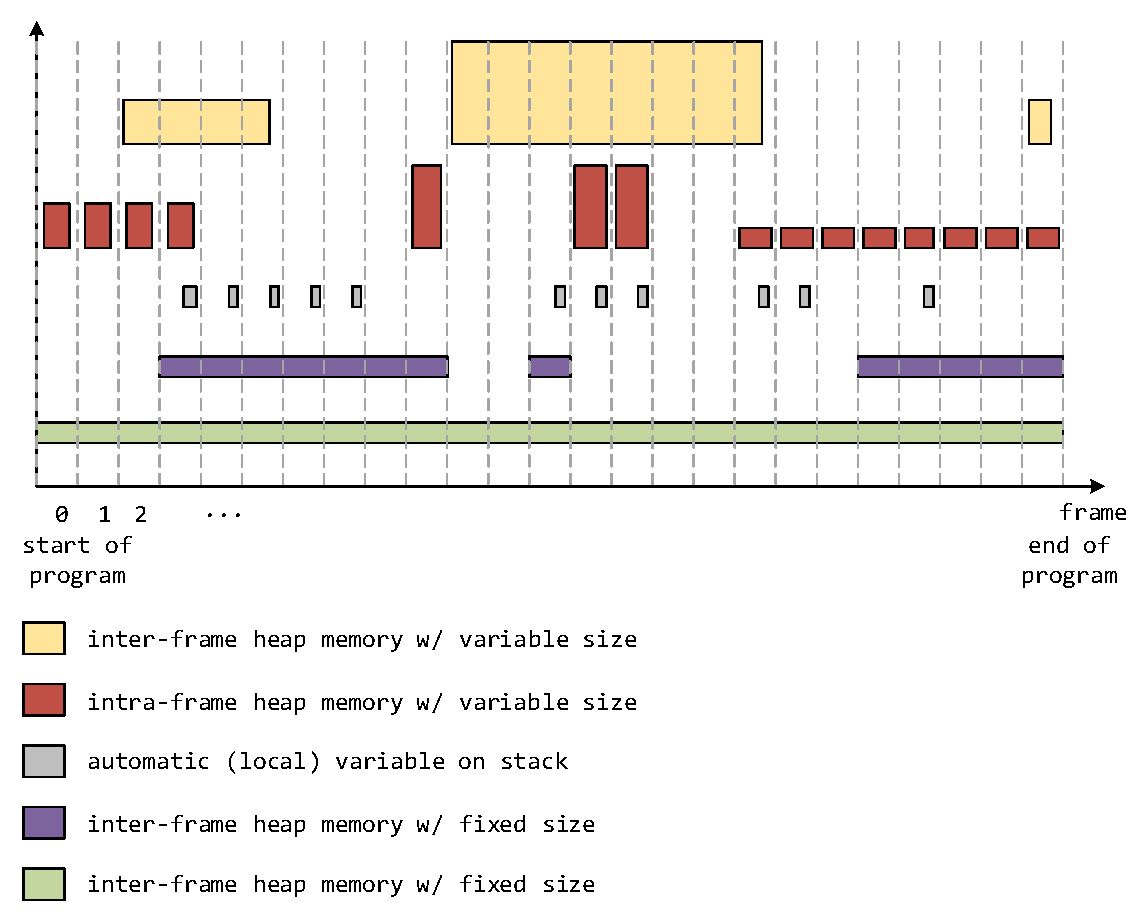
\includegraphics[width=\textwidth]{wmc_tool_ram_memory_types}
\end{center}
\caption{Memory types tracked by the WMC tool}
\label{fig:wmc_tool_ram_memory_types}
\end{figure}

Besides the maximum total intra-frame heap memory and the maximum total inter-frame heap memory the WMC tool also calculates the maximum total \textbf{RAM} memory. This is done under the assumption that both stack and heap are part of a single physical memory block. The WMC tool calculates the total RAM size by adding the current stack size to the heap size of all allocated memory blocks. The total RAM size is calculated during all stack and heap operations. After calculating the total RAM size the WMC tool potentially updates the maximum total RAM size if it has been exceeded and saves the index of the current frame. The process of calculating the total RAM size and the maximum total RAM size is illustrated in Fig:\ref{fig:wmc_tool_max_ram}. 

\begin{figure}[hbtp]
\begin{center}
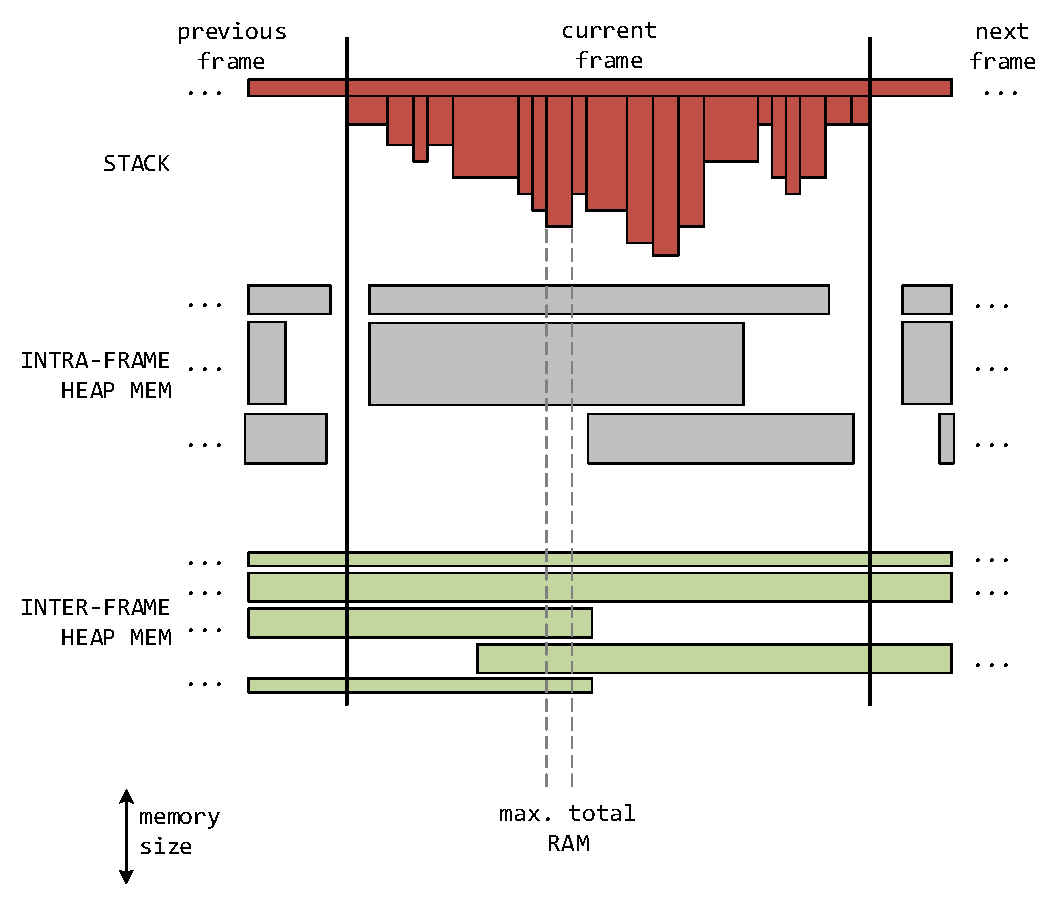
\includegraphics[width=\textwidth]{wmc_tool_max_ram}
\end{center}
\caption{Maximum RAM estimation}
\label{fig:wmc_tool_max_ram}
\end{figure}

It can be seen from Fig:\ref{fig:wmc_tool_max_ram} that the WMC tool doesn't assume that a memory block is allocated or de-allocated at the beggining of the frame or at the end of the frame. The allocation or de-allocation of memory can be done at any time during the processing of the current frame. Note, that in the example of Fig:\ref{fig:wmc_tool_max_ram} the current frame is in fact the worst case where maximum total RAM is reached. This is only to illustrate the memory-tracking mechanism within the WMC tool.

%-----------------------------------------------------------------------------
\subsection{Printing statistics about memory consumption}
\label{ch:printing_statistics_about_memory_consumption}

In order to calculate and print the statistics about RAM and ROM memory consumption in the codec some extra instrumentation needs to be added be the user to the project. The memory counting mechanism must be first initialized with the \verb|reset_mem()| system function. The \verb|reset_mem()| system function is usually called during the initialization phase of the codec, i.e. \textbf{before} the main loop in which individual frames of input data are processed. The \verb|reset_mem()| function takes one input parameter which is an integer value specifying the unit in which memory is calculated and reported. The following list shows all possible values.

\begin{Verbatim}[fontsize=\small]
    USE_BYTES = 0,
    USE_16BITS = 1,
    USE_32BITS = 2
\end{Verbatim}

The user may request that memory is measured in "Bytes", "16b Words" or "32b Words". In Section \ref{ch:printing_statistics_about_computational_complexity}, describing how to print the statistics about computational complexity, the system function \verb|update_wmops()| shall be included at the end of the main loop for processing input data frames. There is a similar system function \verb|update_mem()| which is needed by the memory counting mechanism. However, the \verb|update_mem()| system function is already called as part of the \verb|update_wmops()|. Therefore, there is no need to add this function if \verb|update_wmops()| is already added in the source code. The statistics about memory consumption are printed with the system function \verb|print_mem()| that must be added by the user \textbf{after} the main loop processing input data frames. The function \verb|print_mem()| has one input argument which is the array \verb|ROM_Size_Lookup_Table Const_Data_PROM_Table[]|. Each element in the array is of type \verb|ROM_Size_Lookup_Table| defined in the WMC tool as follows.

\begin{Verbatim}[fontsize=\small]
typedef struct ROM_Size_Lookup_Table
{
    const char file_spec[255];
    int PROM_size;
    int ( *Get_Const_Data_Size_Func )( void );
} ROM_Size_Lookup_Table;
\end{Verbatim}

Thus, each element in the \verb|Const_Data_PROM_Table[]| array is essentially a structure with the following three elements

\begin{itemize}
  \item \verb|file_spec|: string representing the file specification on the command line, e.g. \verb|./codec_lib/*.c|
  \item \verb|PROM_size|: total Program ROM size measured for all source file matching \verb|file_spec|
  \item \verb|Get_Const_Data_Size_Func|: callback function returning the total Const Data (Table) ROM size measured for all source file matching \verb|file_spec|
\end{itemize}

The WMC tool may generate the \verb|Const_Data_PROM_Table[]| array and fill it with the appropriate contents automatically by specifying \verb|-m| o the command line. The user only needs to provide the \verb|.c| source filename in which he has inserted the \verb|print_mem()| function. Thus, the memory instrumentation process can be summarized as follows. The user first needs to insert the functions \verb|reset_mem()| and \verb|print_mem()| in the \verb|.c| source file containing the main loop processing input data frames. Let's assume, for example, that the main file is named as \verb|my_main_codec.c| and that the user has already inserted the appropriate system functions. 

\begin{Verbatim}[fontsize=\small]
int main(void)
{
    FILE *fp;
    int frame = 0;
    
    initilize_codec();
    reset_wmops();
    reset_mem(USE_32BITS);

    while( fread(data, sizeof(short), N_SAMPLES, fp))> 0 )
    {
        /* process the current frame */
        process_current_frame(data);
        ...
        
        frame++;
        update_wmops();
    }

    print_wmops();
    print_mem();
    
    return 0;
}
\end{Verbatim}

The WMC tool shall then be invoked with the \verb|-m| command-line option. As an example, let's assume that the \verb|.c| source files of the project are located in two folders, \verb|./source| and \verb|./lib_smoothing|. The user shall instrument his project by running the WMC tool with: \verb|wmc_tool -m my_main_codec.c ./source/*.c ./lib_smoothing/*.c|. This insert the following instrumentation information in the file \verb|my_main_codec.c|.

\begin{Verbatim}[fontsize=\small]
/*AddedByWMC_Tool*/#ifdef WMOPS
/*AddedByWMC_Tool*/extern int Const_Data_Size_lp_filter(void);
/*AddedByWMC_Tool*/static int Get_Const_Data_Size_source_c(void)
/*AddedByWMC_Tool*/{
/*AddedByWMC_Tool*/    int total_size = 0, sz;
/*AddedByWMC_Tool*/    Get_Const_Data_Size(fft, &sz); total_size += sz;
/*AddedByWMC_Tool*/    Get_Const_Data_Size(hysteresis_filter, &sz); total_size += sz;
/*AddedByWMC_Tool*/    Get_Const_Data_Size(mod_spectrum, &sz); total_size += sz;
/*AddedByWMC_Tool*/    return total_size;
/*AddedByWMC_Tool*/}
/*AddedByWMC_Tool*/ROM_Size_Lookup_Table Const_Data_PROM_Table[] =
/*AddedByWMC_Tool*/{
/*AddedByWMC_Tool*/    { "./source/*.c", 21856, Get_Const_Data_Size_source_c },
/*AddedByWMC_Tool*/    { "./lib_smoothing/*.c, 8954, Const_Data_Size_lp_filter },
/*AddedByWMC_Tool*/    { "", -1, NULL }
/*AddedByWMC_Tool*/};
/*AddedByWMC_Tool*/#endif

int main(void)
{
    FILE *fp;
    int frame = 0;
    
    initilize_codec();
    reset_wmops();
    reset_mem(USE_32BITS);

    while( fread(data, sizeof(short), N_SAMPLES, fp))> 0 )
    {
        /* process the current frame */
        process_current_frame(data);
        ...
        
        frame++;
        update_wmops();
    }

    print_wmops();
    print_mem(Const_Data_PROM_Table);
    
    return 0;
}
\end{Verbatim}

Note, that the WMC tool recognized two file specifications on the command-line and generated an array with two entries. The first entry corresponds to \verb|./source/*.c| and the second entry corresponds to \verb|./lib_smoothing/*.c|. The program ROM is calculated for the source file matching the file specifications and written directly in the lookup table. For Const Data (Table) ROM, the memory size cannot be calculated at the instrumentation stage. Instead, the WMC tool inserts auxiliary functions calculating the memory size in the runtime. In the example above there is only one |.c| source file in the folder \verb|./lib_smoothing/*.c| containing some constant data, \verb|lp_filter.c|. As a result, the WMC tool inserts the callback function \verb|Const_Data_Size_lp_filter()| to retrieve its ROM size. In the folder \verb|./source/*.c| there are three \verb|.c| files containing some constant data, \verb|fft.c|, \verb|hysteresis_filter.c| and \verb|mod_spectrum.c|. The WMC tool creates a wrapper function named \verb|Get_Const_Data_Size_source_c()| in which callback functions are inserted retrieving ROM sizes of the individual source files. The total ROM size is then calculated by summing the individual ROM values and returned by the wrapper function. Finally, the reference to the generated array \verb|Const_Data_PROM_Table[]| is inserted as an argument to the \verb|print_mem()| function. 

It's recommended to use the system functions for resetting, updating and printing of statistics about computational complexity together with the system functions for resetting and printing of statistics about memory consumption. An exemplary printout of the memory consumption may look like this. 

\begin{Verbatim}[fontsize=\small]
Program ROM size (./source/*.c): 21856 instruction words
Program ROM size (./lib_smoothing/*.c): 8954 instruction words
Table ROM (const data) size (source/*.c): 13875 words
Table ROM (const data) size (lib_smoothing/*.c): 6687 words
Maximum RAM (stack + heap) size: 49285 words in frame 1432
Maximum stack size: 27027 words in frame 1432
Maximum intra-frame heap size: 0
Maximum inter-frame heap size: 22258 words in frame 0
\end{Verbatim}

The information about units in which memory consumption is reported is shown at the end of the printout which is not seen in the above example.

With \verb|WMOPS| active it is possible to print detailed statistic about memory consumption in the codec by defining the symbolic constant \verb|MEM_COUNT_DETAILS| in the file \verb|wmc_auto.h|. As part of the detailed printout the user should see the list of functions that were triggered when the maximum stack size has been reached. Furthermore, the detailed memory analysis contains the list of all allocated inter-frame and intra-frame memory blocks when the maximum heap size has been reached. This is illustrated in the following exemplary printout.

\begin{Verbatim}[fontsize=\small]
Function Name     Line   Type Function Parameters          Maximum Size  Usage
------------------------------------------------------------------------------

alloc_filter()     177 malloc length * sizeof(float )        2545 words    99%
smooth_process()   182 malloc sizeof( SMOOTH_STRUCT )          13 words    98%
smooth_process()   715 malloc N_FILT * sizeof(float)        4x895 words    82%
create_head()      749 malloc L_HEAD_N * sizeof(int16_t) )    840 words    90%
\end{Verbatim}

The detailed printout contains the information about the function from which \verb|malloc()| or \verb|calloc()| has been called, the line number and the string describing the size that has been allocated. For each memory block the WMC tool prints the maximum heap size that has been reached and the average usage of the memory block. If the usage is lower than 100\% it means that the allocated memory block has not been fully used in the runtime. When the same memory block has been allocated multiple times in a frame it will be indicated in the printout with the \verb|Nx| prefix where \verb|N| indicates the number of occurences per frame.

Activating \verb|MEM_COUNT_DETAILS| also allows for using the \verb|export_mem()| function in the source code. The function \verb|export_mem()| exports the memory size of all inter-frame and intra-frame memory blocks allocated on heap in the current frame. Therefore, the this function should ideally be inserted \textbf{inside} the main loop processing the input frames, for example as its last statement, similarly as the function \verb|update_wmops()|. The function \verb|export_mem()| takes one input argument which is the pathname to the \verb|.csv| file where the values are to be exported. 


%-----------------------------------------------------------------------------
\section{Limitations}
\label{ch:limitations}

%-----------------------------------------------------------------------------
\subsubsection{MAC detection}

The WMC tool cannot recognize all Multiply-and-ACcumulate (MAC) operations. This would require the expansion of all expressions resembling mathematical formulas which is beyond the scope of the WMC tool. The operation-counting mechanism within the WMC tool recognizes scenarios where either an addition or subtraction is directly followed by a multiplication. For better understanding, see the following examples.

\begin{table}[ht]
\centering
\caption{Detection of MAC operations}
\begin{tabular}{|p{0.5\textwidth}<{\raggedright}|p{0.4\textwidth}<{\raggedright}|}
\hline
\textbf{Instrumented code} & \textbf{Comments} \\
\hline
\verb|$("+=*") sum += sig[i] * filter[i];| & Counted as \verb|MAC(1)| \\
\hline
\verb|$("*-")  d = a * b + c;| & Counted as \verb|MAC(1)| \\
\hline
\verb|$("*/+")  e = a * b / c + d;| & Counted as \verb|MULT(1)|, \verb|DIV(1)| and \verb|ADD(1)| \\
\hline
\end{tabular}
\label{tab:detectiuon_of_mac}
\end{table}

%-----------------------------------------------------------------------------
\subsubsection{Macros}

The WMC tool does not instrument \verb|#define| macros. Local macros will be detected but not instrumented. Macros defined in external files and included with the \verb|#include| directive are not detected as the WMC tool does not open the included files. Such macros are considered as function calls by the WMC tool and instrumented as such. This could eventually lead to compilation errors.

%-----------------------------------------------------------------------------
\subsubsection{Pointer arithmetics}

The WMC tool does not recognize pointer operations because it cannot understand data types. All operations with pointers are treated as mathematical operations. By default, arithmetic operations on pointers such as "\verb|++|" and "\verb|--|" are not instrumented regardless whether they appear as a standalone statement (e.g. \verb|cnt++|) or as part of a complex expression (e.g. \verb|x += a * b + c++|).

%-----------------------------------------------------------------------------
\subsubsection{Moves}

The WMC tool does not distinguish assignations of values to local variables from data moves within a memory block. The assignation operator "\verb|=|" is always intrumented as \verb|$("M")| which is the same as \verb|MOVE()|. Note, that operators such as "\verb|%=|", "\verb|+=|", "\verb|/=|" and similar are instrumented and counted as a single "\verb|%|", "\verb|+|", "\verb|/|" operation, respectively. The \verb|STORE()| macro is not used by the WMC tool.

%-----------------------------------------------------------------------------
\subsubsection{Indirections}

Accessing array members with indices defined as local variables is not counted towards computation complexity if the resulting value is used in a mathematical operation, for example \verb|sum += sign[i] * filt[i]|. For all other cases a \verb|MOVE| operation is counted with \verb|$("M")| such as in the following example \verb|tmp = table[idx]|. The WMC tool does not penalize the access to array members through with brackets "\verb|[]|" even when used in function arguments. However, the WMC tool penalizes the access to structure members either with the "\verb|.|" operator or the "\verb|->|" operator. For example, \verb|T_fruit_struct.color| and \verb|ptr_fruit_struct->color| will be instrumented with \verb|$(".")| and \verb|$("->")|, respectively.

%-----------------------------------------------------------------------------
\subsubsection{Conditional Compilation}

The WMC tool ignores all conditional preprocessor directives, e.g. \verb|#ifdef|, \verb|#else| and \verb|#endif|. Source code which is enclosed by directives for conditional compliation is instrumented regardless of their value (active or inactive). The WMC tool does not support expressions that are separated by directives for conditional compilation. This is illustrated in the following examples.

\begin{table}[ht]
\centering
\caption{Conditional preprocessor directives}
\begin{tabular}{|p{0.34\textwidth}<{\raggedright}|p{0.34\textwidth}<{\raggedright}|p{0.25\textwidth}<{\raggedright}|}
\hline
\textbf{Original source code} & \textbf{Seen by the WMC tool as} & \textbf{Comments} \\
\hline
\begin{BVerbatim}[baseline=t,fontsize=\small]
Fct_Call(arg1, arg2
#ifdef EXTRA_ARG
, arg3, arg4);
#else
, arg3);
#endif

\end{BVerbatim} 
& 
\begin{BVerbatim}[baseline=t,fontsize=\small]
Fct_Call(arg1, arg2
, arg3, arg4);
, arg3);

\end{BVerbatim} 
& Not supported by the WMC tool because of parenthesis imbalance \\
\hline
\begin{BVerbatim}[baseline=t,fontsize=\small]
#ifdef EXTRA_ARG
Fct_Call(arg1, arg2, arg3);
#else
Fct_Call(arg1, arg2);
#endif

\end{BVerbatim} 
& 
\begin{BVerbatim}[baseline=t,fontsize=\small]
Fct_Call(arg1, arg2, arg3);
Fct_Call(arg1, arg2);

\end{BVerbatim} 
& Instrumented as two function calls with three and two arguments, respectively \\
\hline
\begin{BVerbatim}[baseline=t,fontsize=\small]
Fct_Call(arg1, arg2, arg3
#ifdef EXTRA_ARG
, arg4
#endif
);

\end{BVerbatim} 
& 
\begin{BVerbatim}[baseline=t,fontsize=\small]
Fct_Call(arg1, arg2, arg3
, arg4
);

\end{BVerbatim} 
& Instrumented as one function call with four arguments regardless of \verb|EXTRA_ARG| \\
\hline
\begin{BVerbatim}[baseline=t,fontsize=\small]
Fct_Call(arg1, arg2,
#ifdef EXTRA_ARG
, arg3, arg4
#else
, arg3
#endif
);

\end{BVerbatim} 
& 
\begin{BVerbatim}[baseline=t,fontsize=\small]
Fct_Call(arg1, arg2,
, arg3, arg4
, arg3
);

\end{BVerbatim} 
& Instrumented as one function call with five arguments regardless of \verb|EXTRA_ARG| \\
\hline
\end{tabular}
\label{tab:conditional_preprocessor_directives}
\end{table}

It is recommended to use the directives for conditional compilation by enclosing the complete function calls rather than their parts. The limitation is due to the fact that the WMC tool does not evaluate the macros used by the directives (e.g. \verb|EXTRA_ARG| in the examples above). However, during the runtime process the instrumentation of inactive parts in the source code should not have an impact on the estimated complexity. 
